\documentclass{article}

\usepackage{amsmath,amssymb}
\usepackage{tikz}
\usepackage{pgfplots}
\usepackage{xcolor}
\usepackage[left=2.1cm,right=3.1cm,bottom=3cm,footskip=0.75cm,headsep=0.5cm]{geometry}
\usepackage{enumerate}
\usepackage{enumitem}
\usepackage{marvosym}
\usepackage{tabularx}
\usepackage{multirow}
\usepackage[colorlinks = true, linkcolor = blue, urlcolor  = blue, citecolor = blue, anchorcolor = blue]{hyperref}
\usepackage{ulem}

\usepackage{listings}
\definecolor{lightlightgray}{rgb}{0.95,0.95,0.95}
\definecolor{lila}{rgb}{0.8,0,0.8}
\definecolor{mygray}{rgb}{0.5,0.5,0.5}
\definecolor{mygreen}{rgb}{0,0.8,0.26}
\lstdefinestyle{R} {language=R}
\lstset{language=R,
	basicstyle=\ttfamily,
	keywordstyle=\color{lila},
	commentstyle=\color{lightgray},
	stringstyle=\color{mygreen}\ttfamily,
	backgroundcolor=\color{white},
	showstringspaces=false,
	numbers=left,
	numbersep=10pt,
	numberstyle=\color{mygray}\ttfamily,
	identifierstyle=\color{blue},
	xleftmargin=.1\textwidth, 
	%xrightmargin=.1\textwidth,
	escapechar=§,
}

\usepackage[utf8]{inputenc}

\renewcommand*{\arraystretch}{1.4}

\newcolumntype{L}[1]{>{\raggedright\arraybackslash}p{#1}}
\newcolumntype{R}[1]{>{\raggedleft\arraybackslash}p{#1}}
\newcolumntype{C}[1]{>{\centering\let\newline\\\arraybackslash\hspace{0pt}}m{#1}}

\newcommand{\E}{\mathbb{E}}
\DeclareMathOperator{\rk}{rk}
\DeclareMathOperator{\Var}{Var}
\DeclareMathOperator{\Cov}{Cov}
\DeclareMathOperator{\SD}{SD}
\DeclareMathOperator{\Cor}{Cor}

\title{\textbf{Mensch-Computer-Interaktion, Übung 6}}
\author{\textsc{Henry Haustein}, \textsc{Dennis Rössel}}
\date{}

\begin{document}
	\maketitle
	
	\section*{Aufgabe 6.1: Neue UCD-Iteration durchführen}
	\begin{enumerate}[label=(\alph*)]
		\item Einführen eines \textit{Danke}-Buttons, konkretere Erläuterungen vom Registrierungsprozess
		\begin{enumerate}[label=\arabic*.]
			\item Einloggen/Registrieren (SEQ)
			\begin{enumerate}
				\item E-Mail-Adresse eingeben (SEQ)
				\item Passwort eingeben (SEQ)
				\item Benutzernamen eingeben (SEQ)
			\end{enumerate}
			\item richtige Gruppe finden (SEQ)
			\item Post schreiben und abschicken (ALT)
			\begin{enumerate}
				\item Text überlegen (SEQ)
				\item in das Textfeld klicken (SEQ)
				\item Text schreiben (SEQ)
				\item auf Button \textit{abschicken} klicken (SEQ)
			\end{enumerate}
			\item In bereits veröffentlichten Posts suchen (ALT)
			\begin{enumerate}
				\item Keyword(s) überlegen (SEQ)
				\item in Suchleiste klicken (SEQ)
				\item Begriff(e) eingeben (SEQ)
				\item ENTER drücken (SEQ)
			\end{enumerate}
			\item Antworten erhalten (SEQ)
			\item bedanken (SEQ)
			\begin{enumerate}
				\item \textit{Danke}-Button drücken (ALT)
				\item "Danke" o.ä. schreiben (ALT)
			\end{enumerate}
		\end{enumerate}
		\item keine Änderungen notwendig
		\item \textit{Danke}-Button, eine Praktikumsbörse für die Justus-Persona, in der Unternehmen ihre Praktikas ausschreiben können.
		\item Post mit Danke-Button
		\begin{center}
			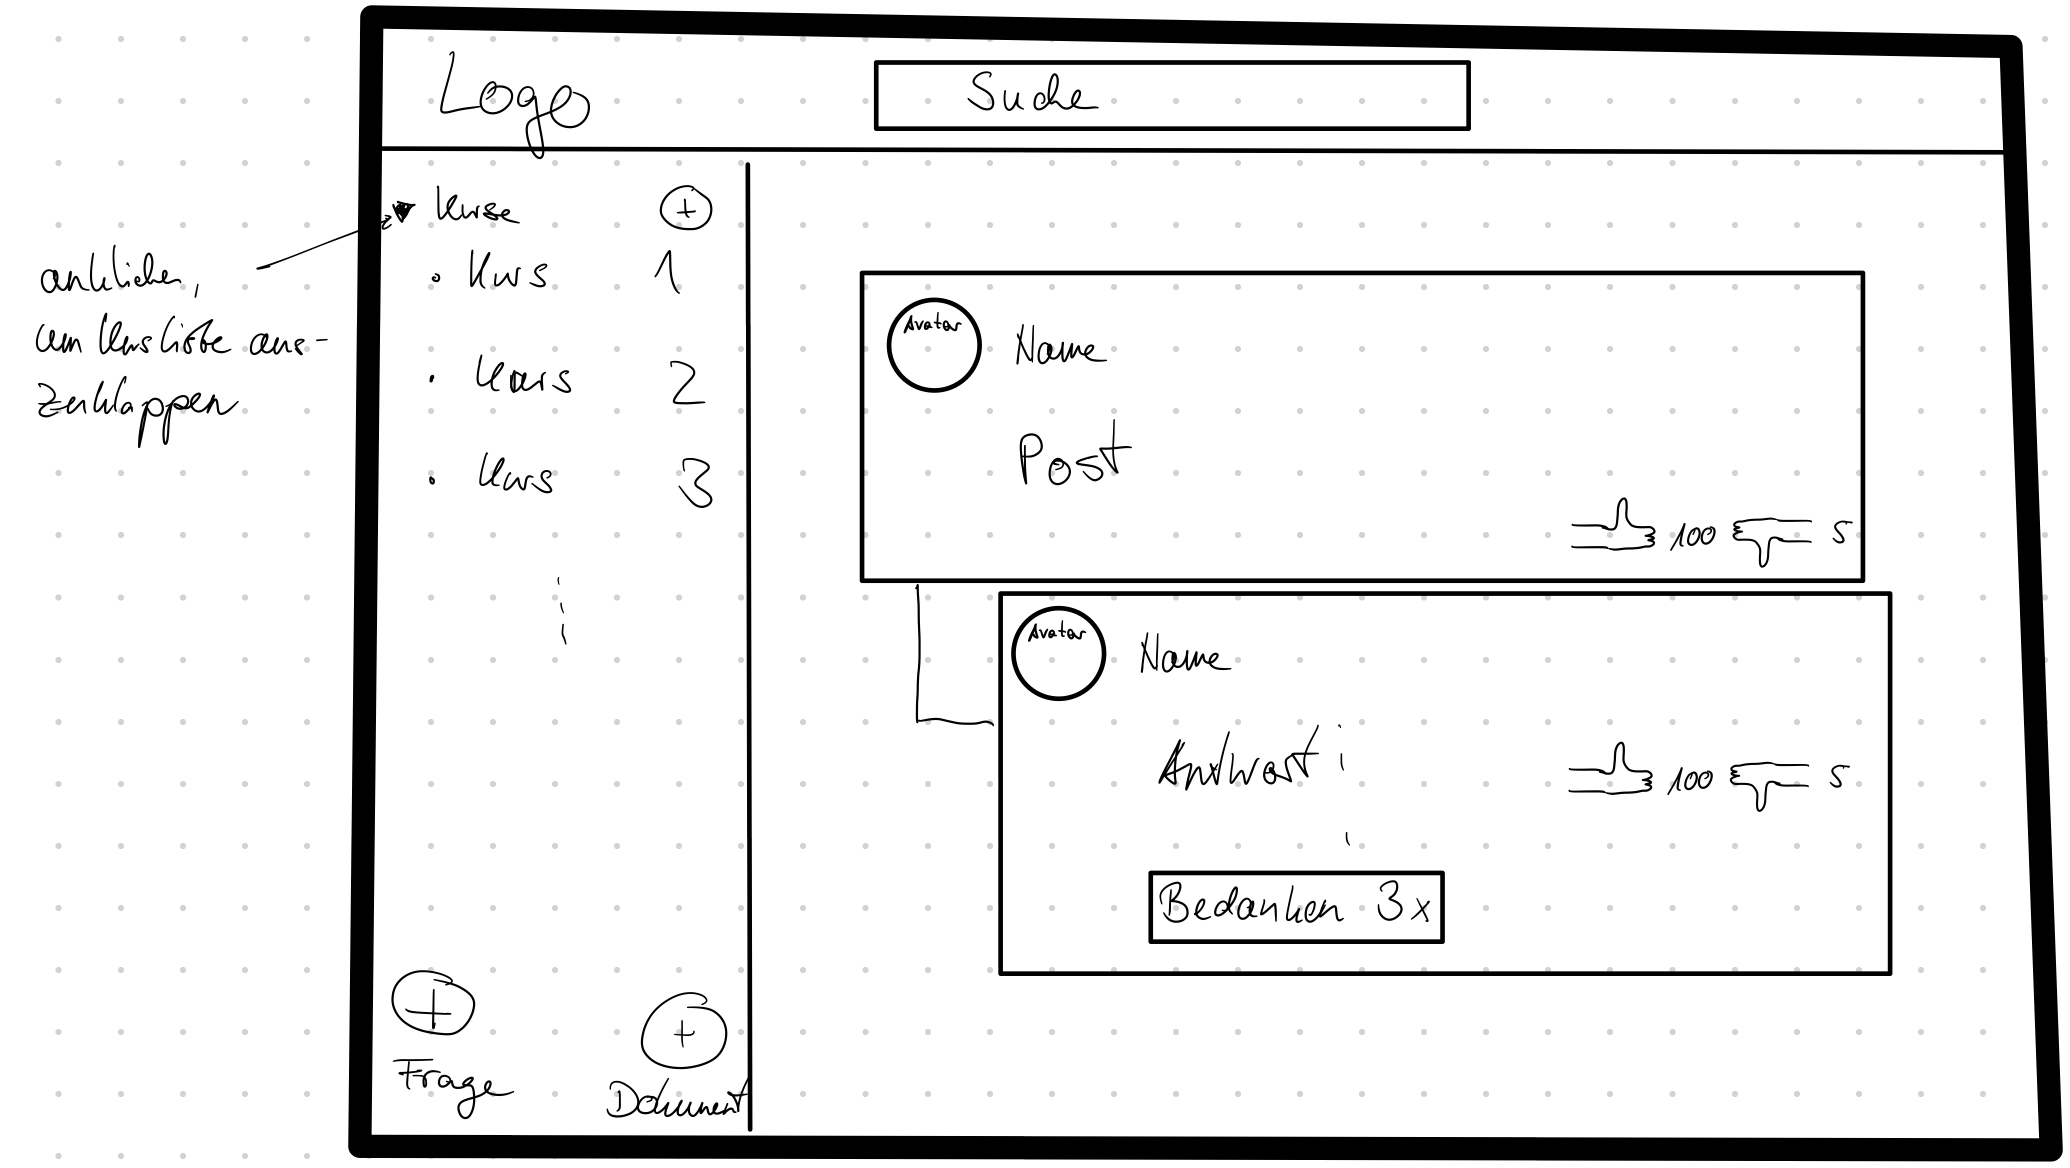
\includegraphics[scale=0.1]{Post-mit-Danke-Button}
		\end{center}
		\item CWT
		\begin{enumerate}[label=\arabic*.]
			\item Benutzer sind unsere Personas, Aufgabe ist es, eine Altklausur zu organisieren, Handlungsfolge siehe (a), Interface ist der Lo-Fi-Prototyp
			\item Ziel ist es Probleme und Uneindeutigkeiten im Interface und in der Bedienung zu finden, während des CWTs wird die Aufgabe abgearbeitet, alle anderen Features der Webseite werden nicht bearbeitet, vorgeschlagene Regeln sind gut, einer von uns beiden ist der Leiter, die Rolle der Persona nimmt ein anderer Student ein, der gut zur Persona passt
			\item Der User hat alle sind Aufgaben erfolgreich abgeschlossen, Buttons waren immer gut sichtbar und erkenntlich, direktes Feedback kam an
			\item es haben sich keine Änderungen ergeben
		\end{enumerate}
	\end{enumerate}
	
\end{document}